%% This is a dissertation template for use with Masters/PhD dissertations at the University of Arizona.
%%
%% This template was created in 2022 by Samuel A. Myers to greatly simplify the existing thesis template.
%% This was done to make the template easier to use, less intimidating, and be because the old template had
%% not been actively updated in over a decade. Furthermore, in recent years the Grad College has greatly
%% relaxed thesis requirmenets, and so the hyperspecific formatting guidelines utilized in the old template
%% were no longer relevant. 
%%
%% Also note that all of the AAS compatability has been explicitly removed, however it can easily be added back
%% by simply including the relevant packages in the preamble. This shouldn't break the template (with the exeption
%% of deluxetable, which is evil and should never be used).
%%
%% This template was made to match the guidelines as listed here (https://arizona.app.box.com/v/grad-gsas-dissformat)
%% in May of 2022. As always, check to make sure that your thesis is compliant before submitting it. If you
%% find any errors, please let the current LPL template manager or grad webmaster know. Furthermore, Be aware that 
%% there are some "secret" requirements that they don't tell you about until you are submitting your thesis. For
%% the most part these should be small things, but if you have problems, reach out to the template manager.
%%
%% This template is based on an existing template that utilized a custom LaTeX class. That template was
%% worked on from the late 80's to early 2000's by a series of graduate students in the Department of
%% Planetary Sciences. Although much of that template has been scrapped, this template is still heavily based
%% on it, and much of their sample text has been utilized. The following is a list of all the students who
%% have worked on various thesis templates.
%%
%% Peter Halverson	1989 (non-LPL)
%% William D. Sears	1994
%% Rov Vervack		1996
%% Andrew Rivkin	1997
%% Joe Spitale		2001
%% Dave O'Brien		2003
%% Ross A. Beyer	2004
%% Jim Richardson	2005
%% Terry Hurford	2005
%% Curtis S. Cooper	2007
%% David A. Minton  2009
%% Samuel A. Myers	2022
%%
%% To compile this template, the recommend run sequence is:
%% PdfLaTeX + Bib(la)tex + PdfLaTeX (x2)
%% This should ensure the references, figures, tables, table of contents, etc are all updated fully and correctly.
%%
%% If you have any questions and its before ~2026, please feel free to email sammyers@arizona.edu


\documentclass[12pt]{report} %Sets default font size and report format



%------------------------------------Import our packages----------------------------------------------

\usepackage[margin=1in]{geometry}	
	%Sets 1in margin on all sides. Required for ProQuest/UMI. Note there are otherwise no margin
	%formatting requirements from the college.
\usepackage{amsfonts,amsmath,amssymb,wasysym}	
	%Includes basic math symbols, including astronomy symbols. Note some symbols may require being
	%placed in their own brakcets to work properly, ie {\odot}
\usepackage{fancyhdr} 							
	%Provides more customization of the headers
\usepackage[explicit]{titlesec}	
	%Allows for cusotmization of section heading appearances						
\usepackage{indentfirst}						
	%By default indents the first line of a paragraph
\usepackage[round]{natbib}						
	%Incredibly useful for citations. The round option puts citations in round instead of square
	%brackets. You can replace this with other packages as you see fit. May require tweaking to
	%get REFERENCES to appear in TOC
\usepackage{graphicx}
	%Package for figure inclusion
\usepackage{caption}
	%Package for manipulating figure captions
\usepackage{hyperref}
	%Governs how hyperlinks are displayed and used
\usepackage{setspace}
	%Allows manipulation of line spacing
\usepackage[titles]{tocloft}
	%Allows manipulation of the table of contents. The titles options ensures changes only apply to the
	%TOC and not the actual title formating in the main document
\usepackage{pdfpages} 
	%Allows inclusion of existing pdfs
\usepackage{bibentry}
	%Allows citing a full reference inline


%--------------------------------------Set up options--------------------------------------------------

%Puts the page number in the upper right hand corner. Note a page number is required on every page except
%the title page and the title page is considered page 1. The location of the page number is optional.
\pagestyle{fancy} 
\fancyhead{} %Clears the default header
\renewcommand{\headrulewidth}{0pt} %Removes header rule line
\fancyhead[R]{\thepage} %Places the page number
\fancyfoot{} %Clears the default footer


%General text formatting
\setlength{\parindent}{1em} %Sets indent length
\setlength{\parskip}{0em} %Sets spacing between paragraphs
\renewcommand{\baselinestretch}{1.5} %Sets line spacing to 1.5
	%Note there are no requirements from the Grad College on these formatting choices
	%They have been set here for readability.

%Link formatting 
\hypersetup{ %Sets color of web and internal links. Can change all to black if you don't want them noticable
    colorlinks=true,
    linkcolor=blue,
    filecolor=magenta,      
    urlcolor=blue,
    pdftitle={UA Dissertation Template}, %Sets the internal file name read by programs like Chrome/Adobe
    pdfpagemode=FullScreen,
    citecolor=blue
}
\urlstyle{same}


%Figure Formatting
%\graphicspath{{"/Users/Wilbur Wildcat/My Figures/"}} %Optional path for where figures are stored
\captionsetup[figure]{labelfont={bf},font=small} %Sets label formatting and font size for figure captions
\captionsetup[table]{labelfont={bf},font=small} %Same as above for table captions


%Chapter/section appearance formating for both numbered and unnumbered chapters, sections, and subsections
\titleformat{\chapter}{\centering\bfseries}{}{0em}{\chaptertitlename{} \thechapter}[\vspace*{1.5ex}#1]
\titleformat{name=\chapter,numberless}{\centering\bfseries}{}{0em}{#1}
\titleformat{\section}{\bfseries}{}{0em}{\thesection\hspace{1em}#1}
\titleformat{name=\section,numberless}{\bfseries}{}{0em}{#1}
\titleformat{\subsection}{\itshape}{}{0em}{\thesubsection\hspace{1em}#1}
\titleformat{name=\subsection,numberless}{\itshape}{}{0em}{#1}


%Table of contents formatting
\renewcommand*\contentsname{TABLE OF CONTENTS} %Renames table of contents
\renewcommand\cftchapdotsep{\cftdotsep} %Inserts dot leader for chapters
\renewcommand{\cftsecfont}{\bfseries} %Bold section titles
\renewcommand{\cftsubsecfont}{\itshape} %Italicize subsection titles
\renewcommand{\cftchappagefont}{\normalfont} %Removes bolding from chapter page numbers
\renewcommand{\cftchapleader}{\normalfont\cftdotfill{\cftsecdotsep}} %Removes bolding for chapter dot leader
\renewcommand\cftchappresnum{\MakeUppercase\chaptername{} } %Prints CHAPTER in front of each chapter
\addtolength\cftchapnumwidth{6em} %Affects spacing between CHAPTER and the chapter name

%Same as above two commands except for appendices
\makeatletter
\g@addto@macro\appendix{
  \addtocontents{toc}{
    \protect\renewcommand{\protect\cftchappresnum}{\MakeUppercase\appendixname{} }
    \addtolength\cftchapnumwidth{1em}
  }
}
\makeatother

%Renames figure and table list
\renewcommand{\listfigurename}{LIST OF FIGURES}
\renewcommand{\listtablename}{LIST OF TABLES}


%Bibliography formatting
\bibliographystyle{abbrvnat} 
	%Sets citation style. Can be replaced as desired. Note that the Grad College does not require a specific
	%format.
\renewcommand{\bibsection}{} %Hides default References title



%---------------------------------------------Custom Values-------------------------------------------------
% These are custom values mainly (exclusively) used to make the title page. Change them as necessary
\newcommand{\CompleteTitle}{How to Construct a Template for a UA Thesis} %The complete title of your dissertation
\newcommand{\FullName}{Gerard Peter Kuiper} %Your full name
\newcommand{\DegreeType}{Doctor of Philosophy} %Your type of degree
\newcommand{\DepartmentName}{Department of Planetary Sciences} %Your department name
\newcommand{\DegreeYear}{2022} %Year of your degree



\begin{document}	%Start the document
\nobibliography* %This is necessary for bibentry to work correctly. If not using bibentry you can comment it out


%---------------------------------------------Title Page--------------------------------------------------
% This page must be formatted as shown here, unless your major does not match the name of your department.
% In this case please refer to the Grad College guidelines. 

\thispagestyle{empty} %Removes page number

\null
\vfill
	%Sets vertical spacing

\begin{center}
\MakeUppercase\CompleteTitle \\ 
\vspace*{1.5em}
by\\
\vspace*{1.5em}
\FullName \\
\vspace*{2em}

\rule{3in}{1pt}\\
\vspace*{-1em}
{\small Copyright \copyright\ \FullName\ \DegreeYear} \\
\vspace*{2em}

A Dissertation Submitted to the Faculty of the\\
\vspace*{1.5em}
\MakeUppercase\DepartmentName \\
\vspace*{1.5em}
In Partial Fulfillment of the Requirements\\
\vspace*{0.5em}
For the Degree of\\
\vspace*{1.5em}
\MakeUppercase\DegreeType \\
\vspace*{1.5em}
In the Graduate College\\
\vspace*{1.5em}
THE UNIVERSITY OF ARIZONA\\
\vspace*{3em}
\DegreeYear
\end{center}

\vfill %Needed for vertical spacing





% ----------------------------------------Approval Page-------------------------------------------------
% Copy the form you need from https://grad.arizona.edu/gsas/dissertations-theses/sample-pages.
% Edit the form in Word as appropriate and save as a pdf. Have your form physically or electronically 
% signed and save it as a pdf. Include it using the following command.

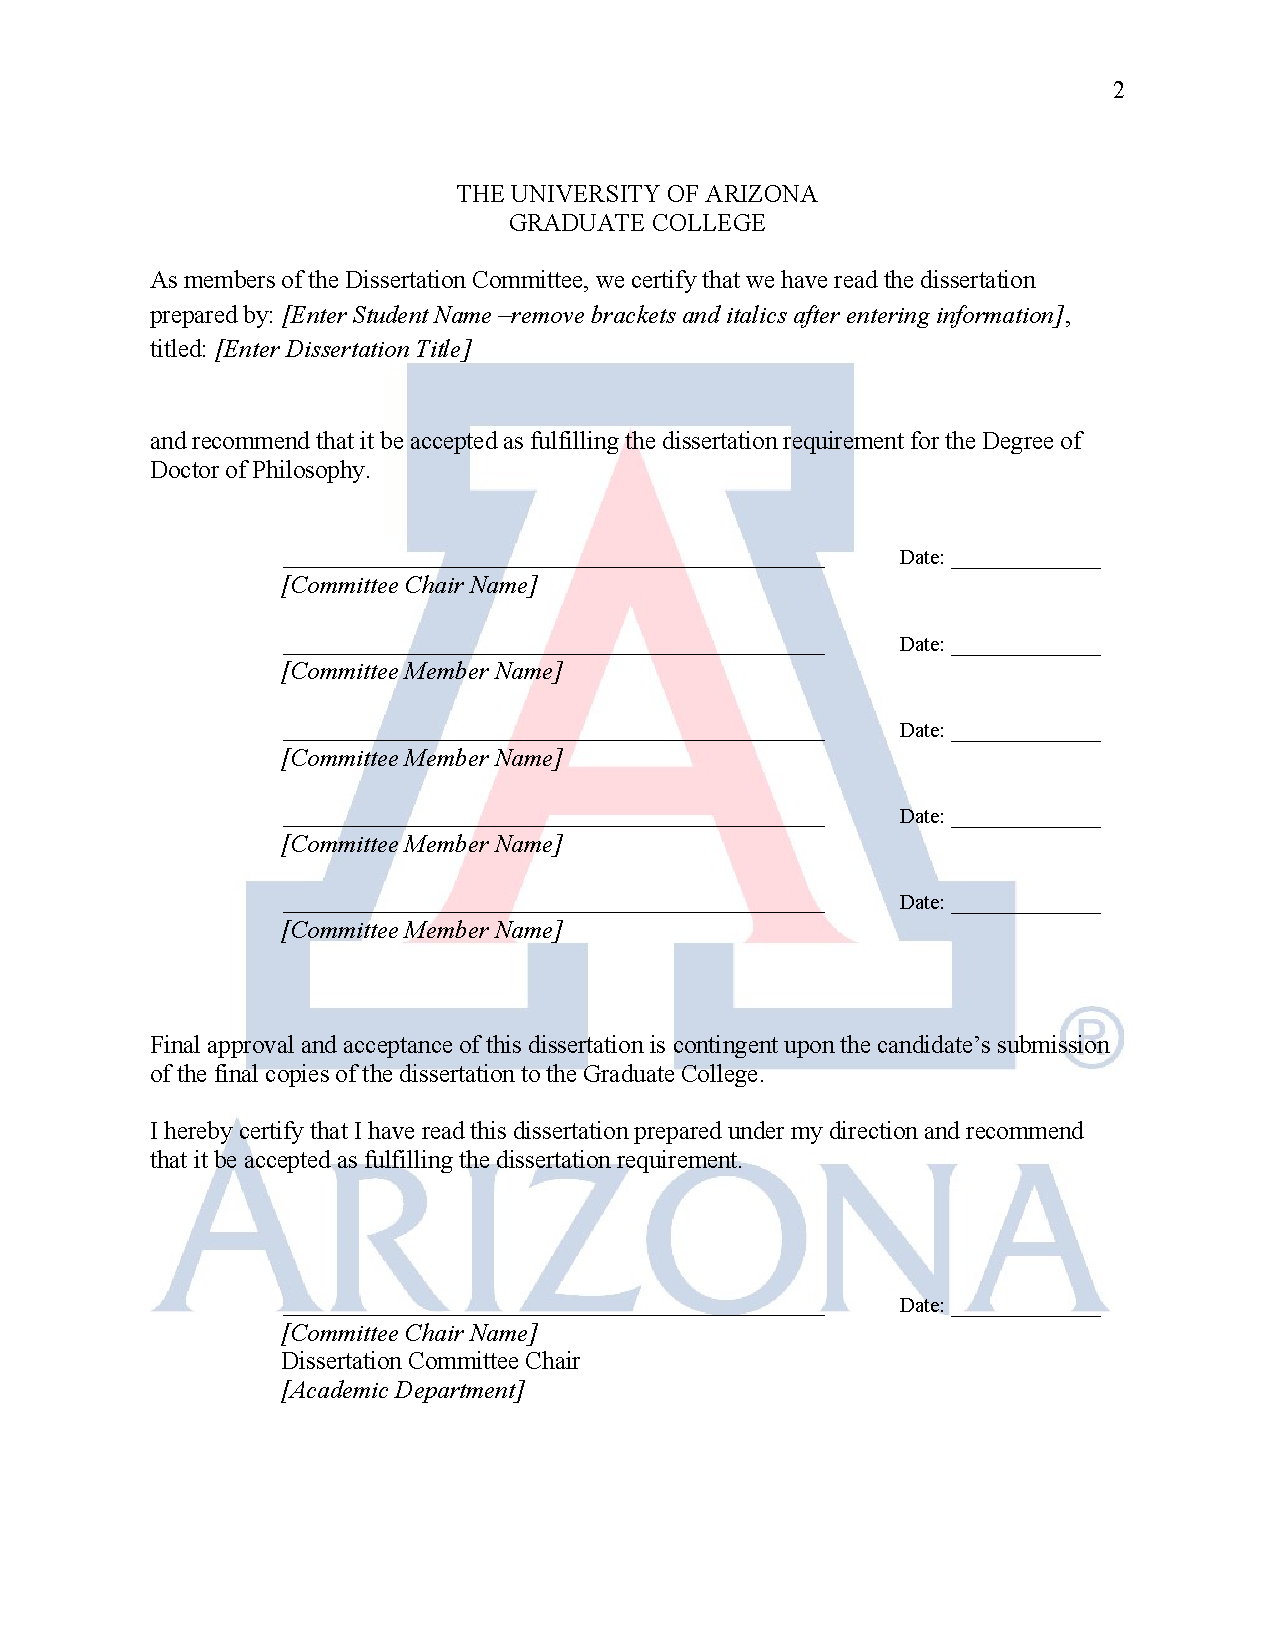
\includepdf[pages={1}]{signed_approval_page.pdf} % Name of signed approval form, in pdf format





%---------------------------------------Acknowledgments------------------------------------------------
% This section is optional. To remove it simply comment out all of the lines betweeen here and the next
% section.
\chapter*{ACKNOWLEDGMENTS}
\thispagestyle{fancy} %Resets custom page number location and first chapter page

Insert your acknowledgments here. They will have the same formatting as the rest of the document. They
should be limited to one page, although this is not explicitly listed in the formatting requirements.





%---------------------------------------Land Acknowledgment------------------------------------------------
% This section is optional. To remove it simply comment out all of the lines betweeen here and the next
% section. Note if you do include, you cannot change any of the wording. If you want to change the wordng
% some students have been allowed to change the title of the chapter to "PERSONAL STATEMENT ON LAND
% ACKNOWLEDGEMENT".
\chapter*{LAND ACKNOWLEDGMENT}
\thispagestyle{fancy} %Resets custom page number location and first chapter page

\noindent We respectfully acknowledge the University of Arizona is on the land and territories of Indigenous peoples.
Today, Arizona is home to 22 federally recognized tribes, with Tucson being home to the O'odham and the Yaqui.
Committed to diversity and inclusion, the University strives to build sustainable relationships with sovereign
Native Nations and Indigenous communities through education offerings, partnerships, and community service.





%----------------------------------------------Dedication------------------------------------------------
% This section is optional. To remove it simply comment out all of the lines betweeen here and the next
% section. This should be limited to one page, although this is not explicitly listed in the formatting
% requirements.
\chapter*{DEDICATION}
\thispagestyle{fancy} %Resets custom page number location and first chapter page

\begin{center}
\textit{Insert your dedication here}
\end{center}





%--------------------------------------Table of Contents--------------------------------------------------
% Note that at all entries in the TOC must be formatted as they are in the text, i.e. if a title is bolded
% in the text it must be bolded in the TOC. This will be done automatically if you don't change any of the
% formating.
\tableofcontents
\thispagestyle{fancy} %Resets custom page number location





%----------------------------------------List of Figures--------------------------------------------------
\cleardoublepage %Ensures accurate page numbering
\phantomsection %Needed for hyperref
\addcontentsline{toc}{chapter}{\listfigurename} %Includes figure list in table of contents
\listoffigures
\thispagestyle{fancy} %Resets custom page number location





%----------------------------------------List of Tables--------------------------------------------------
\cleardoublepage %Ensures accurate page numbering
\phantomsection %Needed for hyperref
\addcontentsline{toc}{chapter}{\listtablename} %Includes table list in table of contents
\listoftables
\thispagestyle{fancy} %Resets custom page number location





%------------------------------------------------Abstract--------------------------------------------------
\chapter*{ABSTRACT}
\thispagestyle{fancy} %Resets custom page number location on page
\addcontentsline{toc}{chapter}{ABSTRACT}

This is where the body of your abstract goes. The abstract should summarize your work. There is no formal 
length limit/requirement that I could find as of the creation of this template.





%----------------------------------------Example Chapter--------------------------------------------------
\chapter{Sample Chapter}
\thispagestyle{fancy} %Resets custom page number location on first chapter page

\section{Introduction}
This is an example of a numbered section. You can also created unnumbered sections and subsections, although
I recommend against it. If you create unnumbered sections you will have to add them to the Table of Contents 
manually with the \texttt{addcontentsline} command. \footnote{By the way footnotes are a thing}.\\

\textit{Note: All titles (chapters, sections, subsections, etc must be in Title Case.)} 

\section*{An Unnumbered Section}
This is an unnumbered section that has not been added to the Table of Contents.

\subsection{Subsections!}
You can also create subsections. They follow the same rules as sections.


\section{Math Example}
This is a real short example of using the equation environment.

\begin{equation}
	y = mx + b
\end{equation}

There is an awful lot that the equation environment and math mode can do for you.


\section{References}
Here is an example of references using the natbib package. You can reference in a number of ways.  The
ones that are most useful are parenthetical \citep{article,articletwo} or inline, as in \citet{articletwo} 
said this or that. You can also include information within the citation \citep[e.g.][doesn't have any
page numbers]{2003jgr}.  You don't even need to have the reference in your text to be included. \nocite{2004LPI}

You can also cite your references directly inline using the \texttt{bibentry} command as follows: \bibentry{article}


\section{Figures} \label{section:figures}
On the next page is a figure inclusion using the `graphicx' package. This puts figures on their own page by 
themselves. They don't need to be on separate pages, there is no requirement that they be on separate pages.
If you want to put a figure on a page with text, don't include the \emph{p!} option in square brackets at 
the begin figure command.

You can use most common file types with this package. Just make sure the file extension listed in the command
matches the actual file.

Also note that the \verb=\caption= command has an optional square-bracketed argument and a curly-bracketed 
argument.  Whatever you put in square brackets will be used as the short caption, and will go into the 
List of Figures.  The stuff in the curly brackets will be placed on the page under your figure.


\begin{figure}[p!]
\begin{center}
\includegraphics{figure.eps}
\caption[Short figure caption for LOF]{Sample figure caption (to appear below
the actual figure). \label{samplefig}}
\end{center}
\end{figure}

You can reference a figure later using the \verb=\label= command (Figure~\ref{samplefig}). This can also be
done for sections and chapters (Section~\ref{section:figures}).





%----------------------------------Example Chapter 2: Electric Boogaloo-----------------------------------------
% You can also use the input command to include separate tex files. Try to avoid the input command as it may 
% break the formatting (or more often just straight up not work).
\chapter{A Pole-to-Pole Pressure-Temperature Map of Saturn's Thermosphere from Cassini Grand Finale Data} 
\thispagestyle{fancy} 

Originally published as: Brown, Z., Koskinen, T., M\"{u}ller-Wodarg-Wodarg, I. et al. A pole-to-pole pressure–temperature map of Saturn’s thermosphere from Cassini Grand Finale data. \textit{Nature Astronomy} 4, 872–879 (2020). doi: 10.1038/s41550-020-1060-0
[* Need to fix the references, add the figures, review the way the sections are set up, and double check the equations and other symbols/math.]

\section{Introduction}
Temperatures of the outer planet thermospheres exceed those predicted by solar heating alone by several hundred degrees. Enough energy is deposited at auroral regions to heat the entire thermosphere but models predict that equatorward distribution is inhibited by strong Coriolis forces and ion drag[1,2]. A better understanding of auroral energy deposition and circulation are critical to solving this so-called energy crisis. Stellar occultations observed by the UVIS instrument during the Cassini Grand Finale were designed to map the thermosphere from pole to pole. We analyze these observations, together with earlier observations from 2016 and 2017, to create a two-dimensional map of densities and temperatures in Saturn’s thermosphere as a function of latitude and depth. The observed temperatures at auroral latitudes are cooler and peak at higher altitudes and lower latitudes than predicted by models, leading to a shallower meridional pressure gradient. Under modified geostrophy[3], we infer slower westward zonal winds that extend to lower latitudes than predicted, supporting equatorward flow from approximately 70° to 30° latitude in both hemispheres. We also show evidence of atmospheric waves in the data that can contribute to equatorward redistribution of energy through zonal drag.

Cassini observed the Grand Finale suite of more than 30 stellar occultations in the UVIS far ultraviolet (FUV) and extreme ultraviolet (EUV) channels between June 24th and August 4th, 2017. These observations probe different longitudes and local times at latitudes from 86° S to 86° N, including over a dozen at polar latitudes. We analyze 23 EUV occultations with sufficient data quality to allow for accurate H\sub{2} density and temperature retrieval along with 10 previously unpublished observations from 2016 and earlier in 2017 (Fig. 1a, Supplementary Table 1). These data probe pressures from $\sim$0.1 $\mu$bar to $\sim$1 picobar, corresponding to equatorial altitudes of $\sim$1,000 to $\sim$3,000 km above the 1 bar level (see Methods).

\section{Results and Discussion}

We fit H\textsubscript{2} density profiles above the altitude of 1,700-1,800 km to retrieve exospheric temperatures as a function of latitude (Fig. 1b). From $\sim$30˚ to $\sim$65˚ latitude, temperature increases from 394 to 513 K in the south and from 340 K to 586 K in the north, consistent with previously published results from Cassini[4] and Voyager[5] occultations. At polar latitudes, the temperature decreases with latitude from 513 K to 373 K between 61˚ S and 86˚ S, and from 586 K to 437 K between 66˚ N and 86˚ N. The Voyager data point at 82˚ S was previously considered an outlier[5] but now agrees well with the observed polar temperature minima. Our temperatures also agree roughly with the temperatures inferred from column-integrated H\textsubscript{3}\textsuperscript{+} observations[6,7]. The magnitude of temporal and longitudinal variations in temperature is limited by the standard deviation, which we infer for 15° latitude bins over the course of the mission. This standard deviation ranges from 11 to 56 K, with the largest value at 30-45˚ N, reflecting a greater temporal variability at those latitudes (Supplementary Figure 1).

We compare the observed temperatures to those predicted by the Saturn Thermosphere-Ionosphere general circulation model[1,2] (Fig. 1b), the only current model of Saturn’s thermosphere to include both global circulation and the response to auroral and solar heating. The most recent version of the model (hereafter, the STIM 2019 model) applies zonal drag in the momentum equation to slow down westward jets at high latitudes and allow for the redistribution of auroral energy to match the observed low-latitude temperatures. At polar latitudes, the STIM 2019 model predicts that temperature further increases with latitude or remains flat. While the cool polar temperatures differ from model predictions, similar temperatures observed in the north and south agree with the seasonal trend predicted by the STIM 2019 model for northern summer solstice (May 24, 2017). Additional heating in the southern hemisphere from the northward shift of Saturn’s magnetic field[8] offsets the larger Joule heating derived from greater photo-ionization in the northern summer hemisphere, an effect which has also been observed in H\textsubscript{3}\textsuperscript{+} temperatures[9].

The polar temperature minima are difficult to explain in the context of existing models. Joule heating due to auroral currents is expected to be the main heating mechanism at high latitudes. The magnetospheric electric field that drives the predicted auroral currents, however, is constrained to latitudes of $\sim$65 - 90˚ by ionosphere-magnetosphere interactions and falls to zero inside the polar cap. Therefore, dynamics is predicted to redistribute energy from the auroral oval towards the poles, leading to the higher than observed temperatures inside the polar caps. In terms of cooling mechanisms, radiative cooling is unlikely to play a role in the polar energy balance. This is because we probe altitudes above the homopause, where the abundance of species heavier than H\textsubscript{2} that could contribute significantly to radiative cooling is low. Also, H\textsubscript{3}\textsuperscript{+} cooling that is important on Jupiter[12,13,14] is expected to be negligible on Saturn[2]. This means that dynamics, in combination with the auroral electric fields, is still the likely driver of the observed polar temperatures. The zonal winds that we infer from the data extend to lower latitudes than predicted and as a result, the poleward meridional winds are also shifted to lower latitudes (see below). This implies that poleward transport is less efficient than expected. Adiabatic cooling due to polar upwelling would also help to cool the poles, although the data are not sufficient to confirm this. Our results call for a revision of the existing models to properly explain the polar temperature structure, particularly the shift of the observed temperature peak from the predicted location.

By interpolating over the observed temperature profiles, we create a latitude-pressure contour (Fig. 2a) and compare the results with the STIM 2019 model (Fig. 2b). The observed temperatures at low latitudes are similar to model predictions ($\sim$ 150-420 K), however, the data differs from the model at higher latitudes. The highest temperatures in the model are located at the poles at a pressure of about 10-8 bar, with maximum values higher than 650 K. The observations show a cooler maximum temperature ($\sim$ 550 K), located higher in the atmosphere and at lower latitudes than the STIM 2019 model predicts, resulting in shallower meridional pressure gradients. This has implications for winds.

We use the data to infer winds at three pressure levels (10, 1 and 0.1 nbars) under modified geostrophy in oblate spheroidal coordinates[3,15], assuming a balance between ion drag, pressure gradient, and Coriolis forces[3]. The wind equations are populated with our data-derived geopotential gradients along with electric field and conductivity values identical to those used by STIM 2019, allowing for a direct comparison of the resulting wind fields (see Methods). The inferred zonal winds are close to geostrophic and depend mostly on the gravitational potential gradient on constant pressure levels (Fig. 3a). We infer the radii and latitudes required to calculate the potentials from the observed density and temperature profiles. By fitting a polynomial to the potentials, we determine the potential gradient with latitude and calculate the zonal and meridional winds (see Methods).

The inferred zonal winds exhibit broad, westward jets spanning from 30˚ to the highest latitudes sampled and centered at 60-75˚ latitude at the 1 and 0.1 nbar levels (Fig. 3b). Maximum wind speeds for each level are between 500 and 800 m/s. These jets are driven almost entirely by heating and Coriolis forces. The effect of ion drag can be seen in the small westward enhancements at the 10 nbar level near 75° latitude, corresponding to the sharp peak in auroral electric field and conductivities. Zonal jets predicted by the STIM 2019 model are $\sim$ 10˚ wide, peak near 80˚ latitude and exhibit maximum speeds of $\sim$1,100 m/s in the south and $\sim$1,400 m/s in the north (Fig. 3b). In contrast, the inferred zonal winds are broader, slower and extend to lower latitudes than in the model.

Elevated equatorial potential on each of the sampled pressure levels is consistent with eastward winds at latitudes lower than about 30˚ (Fig. 3b). Winds below this region in the equatorial stratosphere are characterized by Saturn’s quasi-periodic oscillation (QPO): a pair of descending and opposing zonal jets[16] imposed upon a strong background eastward jet[17]. The stratospheric jet persists at least up to the 10 mbar level[18] and our data suggest that it is also present in the thermosphere. We note that our gravitational potential does not take into account the effect of differential rotation which was recently detected in Saturn’s deep interior [19] and is characterized by super- and sub-rotating jets that extend thousands of kilometers below the 1 bar level. While incorporating the refined gravity coefficients that arise from differential rotation could affect the morphology of the elevated equatorial potential, we estimate that it would produce only small changes to the overall wind field that we infer.

The accuracy of our inferred winds depends on the assumption of modified geostrophy, input parameters such as conductivities and electric fields, and the latitude resolution of our data. Neglecting the effect of the model input parameters on derived winds, the uncertainty in zonal geostrophic winds depends on the uncertainty in the gradient of the gravitational potential, which is set by our polynomial fit to the data (Fig. 3a). The uncertainty in the potential itself is small, and is derived from uncertainty in pressure level radii. We calculate pressure with the ideal gas law and propagate the error in number density and temperature to find the uncertainty in pressure[20]. The change in radius corresponding to the uncertainty in pressure is given by the hypsometric equation. We bracket the gravitational potential at each latitude by the potential given by the radius at the isobar plus and minus the uncertainty in radius. The mean uncertainty in radius at the 1 nbar pressure level is 20 km, giving an uncertainty in the potential of less than 0.1 \%. The latitude spacing of our data, however, limits the resolution of the fits and while strong, narrow jets may be present, they are not necessarily detected in the data. Despite our inability to fully resolve the wind structure, it is clear that the jets extend to a lower latitude than in the model and that this arises from the structure of the meridional temperature gradient.

The implied meridional winds diverge near 70˚ latitude, with flows toward the poles and toward the equator down to a latitude of $\sim$30˚ (Fig. 3c). Maximum poleward wind speeds are 30-45 m/s at the 0.1 and 1 nbar levels and 85-110 m/s at the 10 nbar level. The peak equatorward flow speed is 20-40 m/s, depending on the pressure level. We expect the thermosphere to be fed from below at latitudes where meridional winds diverge to support conservation of mass. Flow away from 70˚ latitude suggests the transport of heat to both higher latitudes and to the middle latitudes. This latitude is poleward of the highest observed temperatures and equatorward of 75˚ where average auroral brightness peaks[21].

 In our inferred wind calculations, we neglect viscous and wave drag, which we expect to play a role in circulation. Our assumption of zonal symmetry means that meridional geostrophic winds are zero and therefore only ion drag is available to drive meridional winds. In reality, zonal asymmetries are likely and it is reasonable to expect that we have underestimated meridional wind speeds. A meridional wind pattern similar to the data is predicted by the STIM 2019 model (Fig. 3c), although the winds in the model are in general faster and diverge at a higher latitude than we infer. This indicates that the STIM 2019 model is correct in principle and the drag and heating rates could be adjusted to fit the new data. This adds to the growing evidence contradicting model predictions that Saturn’s strong Coriolis forces and polar ion drag prevent equatorward flow of energy[21].
 
Müller-Wodarg et al.[1] applied different drag parameterizations to match the previously observed temperatures and we use the best fit, case C (see Fig. 2 of that work). They argue that drag could be from momentum deposition by atmospheric waves and conclude that density perturbations observed by the Cassini Ion Neutral Mass Spectrometer (INMS) measurements during Grand Finale deep dips are sufficiently large to account for the required drag. We observe similar wave-like features in temperature in each of the occultations that we analyzed (Fig. 4) with wavelengths of $\sim$100-200 km and amplitudes on the order of 10-50 K at lower altitudes that in some cases increase to 100 K or more near 1,800 km. Signal to noise in transmission, however, decreases rapidly with altitude and wave properties at high altitudes are uncertain. More work is needed to assess how well wave properties can be inferred from occultation data in general, since these observations probe line of sight densities, but in principle we confirm the detection of waves in the thermosphere.

\section{Conclusions}

The pole-to-pole snapshot of Saturn’s thermosphere we created from the Cassini Grand Finale occultation data has several implications for circulation and redistribution of energy, including the polar temperature minima that imply less efficient poleward transport of energy or polar upwelling that is not matched by current models. At low latitudes, inferred zonal winds arising from the gravitational potential gradient along isobars are eastward, echoing observed stratospheric flow. Poleward of 30˚ latitude, we infer slower westward zonal jets that extend to latitudes lower than predicted by models. Our data also support the idea that waves are present globally in the thermosphere and have properties similar to those that can significantly alter global circulation[2]. The results of this study provide evidence for the redistribution of auroral energy to lower latitudes and underline the importance of dynamics in controlling thermospheric temperatures.

\section{Methods}

In general, the Grand Finale occultations are of good quality, obtained with stable pointing and an average altitude sampling resolution of 11 km with the 8.875-s integration time. In this article we refer to occultations by their year, day of year and latitude as designated in Supplementary Tables 1 and 2. Our labels are more concise than those used by the Planetary Data System, which are also listed.

\subsection{Data evaluation and selection}
Of 30 Grand Finale occultations, we analysed 23 and discarded or postponed 7 due to issues with pointing or insufficient data in critical altitude regions. We describe here our methods for ensuring accurate data retrieval and the circumstances leading to each of the observation exclusions. We first inspected detector images and spectra at each time step for anomalies, including evidence of cosmic ray impacts. One in over 11,000 detector images inspected showed evidence of such an anomaly, with all other images demonstrating expected behaviour (greatest signal at the centre of the detector and small changes between subsequent time steps). Next we checked for stable spacecraft pointing during the observations. This is important because detector response is sensitive to the location of the stellar image in the field of view, and drifts in pointing cause time-dependent deviations in observed wavelengths and signal. We found that the majority of Grand Finale occultations are stable. A few of them have periodic drifts of less than 0.06 mrad in the instrument field of view (ST17D182L78S, ST17D185L39N, ST17D198L66N, ST17D202L80S), which are acceptably small. We searched the spectra above the altitude of 1,000 km for shifts in wavelength greater than a few picometres that could prevent accurate H\textsubscript{2} density retrieval. We identified two occultations with substantial wavelength shifts throughout (ST17D178L65S, ST17D201L40S) and decided to postpone their analysis for future work. In six occultations we found large pointing-induced shifts in wavelength that were limited to high altitudes (ST17D194L34S, ST17D195L55S,ST17D195L45S, ST17D201L28S, ST17D202L80S, ST17D209L61S). We analysed these occultations, excluding the regions with poor stability, which do not affect the altitudes of interest.

We excluded two occultations (ST17D182L78S, ST17D196L81N) that were split into sections, probably during downlink. In both occultations, one section covers lower altitudes including the retrieval region and the other section covers high altitudes including the reference region. The observations in each section show slight differences in pointing and further work is needed before they can be analysed. One occultation is missing data between the altitudes of 1,351 and 1,768 km, in the critical retrieval region, and cannot be analysed (ST17D189L50N). Two other observations lack sufficient high-altitude data to provide a robust reference spectrum, with upper altitude limits of 3,121 and 3,350 km (ST17D176L12N, ST17D176L24N). These observations could be analysed by using a reference spectrum from another occultation of the same star, but this results in yet greater difficulties due to pointing differences, and we exclude them from this work. Finally, because of the varying response of the EUV detector to the stable position of the stellar image in the field of view, variations in absolute wavelength also occur between occultations. We determined the wavelength scale for each occultation by cross-correlating the observed transmission spectra with a model spectrum of the H\textsubscript{2} Lyman and Werner absorption bands at altitudes from 1,000 to 1,800 km and then applied this wavelength correction to the other altitudes.

\subsection{Data reduction}
For each occultation, we generate line of sight transmission spectra at individual tangent altitudes by dividing the transmitted spectrum by the unattenuated reference spectrum of the star. Tangent altitudes are defined as the distance along the surface normal to the line of sight from the 1-bar level, which we determine using the Anderson and Schubert21 model. We measure absorption in the Lyman and Werner electronic bands of H\textsubscript{2} between 910 and 1,085 Å. Although the EUV channel observes wavelengths from 580 to 1,180 Å, starlight at wavelengths shorter than 911 Å is almost entirely absorbed by interstellar atomic hydrogen. Because diffusive separation causes the density of species heavier than H\textsubscript{2} to drop off rapidly above the homopause located at 0.01–0.1 μbar (ref. 22), absorption in the EUV channel is dominated by H\textsubscript{2}. Our analysis excludes the lowest altitudes available in the EUV channel, where CH4 begins to contribute to absorption.

To calculate transmission, we designate the following altitude regions for each occultation: (1) the reference region, taken at high altitudes where the observed starlight is unocculted, (2) the retrieval region, where attenuation in the atmosphere results in transmission between 0 and 1, and (3) the background region, where starlight is fully occulted and any observed photons are from non-stellar sources. The reference regions have lower boundaries between 3,500 km and 5,000 km and upper boundaries between 4,000 km and 11,000 km, depending on the occultation. In designating reference regions, we verify that transmission is equal to unity in the strong H\textsubscript{2} absorption band, 960–970 Å, and exclude any regions of unstable pointing. Because methane also absorbs at EUV wavelengths where we measure H\textsubscript{2} absorption, we wish to exclude altitudes where absorption by CH4 is important from the retrieval regions. Hydrocarbon retrievals will be presented in future work. To minimize absorption by CH4, we define the lower limit of the retrieval regions as the higher of (1) the lowest altitude where the running mean over five points in the 960–970-Å band exceeds 2 counts and (2) the lowest altitude with substantial transmission at 1,140–1,150 Å, where CH4 is the main absorber. Finally, we designate the background count region as the altitudes below which both the 960–970-Å band and the 1,140–1,150-Å methane band transmission light curves go to zero (from 450 to 750 km depending on the occultation). Within this region we determine the background counts for each wavelength, taken as the average over the altitudes in the background region. We find small average background counts of 0–10 per wavelength per integration period, which we subtract from the signal at all altitudes.

After these checks, we retrieve the H\textsubscript{2} density and temperature profiles from the transmission time series by using the methods adapted from Koskinen et al.4, which we summarize here. The column density at each tangent altitude is a measure of the total atmospheric H\textsubscript{2} along the line of sight. We retrieve column density using a Levenberg–Marquardt least squares algorithm to fit the observed transmission spectra with a high-resolution transmission model based on the H\textsubscript{2} line lists of Abgrall and colleagues23–25. convolved with the line spread function of the UVIS instrument (see the UVIS User’s Guide available through the Planetary Data System Rings Node), generalized to the EUV channel. Since the absorption cross-section of H\textsubscript{2} in the Lyman and Werner electronic bands depends on temperature (which we are working to derive), we retrieve the column density iteratively, starting with an initial H\textsubscript{2} cross-section at a constant temperature of 300 K.

We invert the column density profiles using Tikhonov regularization and fit a forward-model temperature profile18 to the resulting number density profile. We then re-retrieve column densities, now using H\textsubscript{2} cross-sections that vary with altitude according to the forward-model temperatures from the previous step. This is repeated until subsequent solutions converge (between four and ten iterations). We then invert column density again with Tikhonov regularizationto obtain the final number density profile. Assuming hydrostatic equilibrium and an ideal gas, we also integrate the number density profiles to directly retrieve temperature profiles, which typically agree well with the parameterized forwardmodel temperature profile. The number density profiles above the altitude of 1,700–1,800 km are generally noisy and we smooth the profiles in this region by fitting the data with an exponential power series. Although the relatively large uncertainties prevent us from ruling out high-altitude temperature gradients, the fits are generally consistent with an isothermal atmosphere. Because we expect temperatures to remain constant with altitude out to the exobase at 2,700–3,000 km (ref. 26), we have adopted the common convention of referring to the temperature above 1,700–1,800 km as the ‘exospheric’ temperature. Our results indicate a trend in exothermic temperature with latitude in the auroral regions. Given that auroral brightness is not uniform in local solar time19, we considered the possibility that our latitudinal trend in polar exospheric temperatures might be correlated instead with auroral activity. We find that this trend is not primarily dependent upon local solar time (Supplementary Fig. 2).

Figure 4 shows an example of the direct-inversion and forward-model temperature profiles for an occultation at 86°. We detect wave-like features in temperature in all of the 23 Grand Finale occultations, which constitutes evidence for upwardly propagating gravity waves. Because the average temperature profile resolution is $\sim$20 km in altitude, only waves with wavelengths a few times this distance are detectable. Furthermore, integration along the line of sight means that we can only detect waves with a large horizontal extent. More work is needed to interpret the observations and accurately infer the properties of the detectable waves.

\subsection{Derivation of winds}
We infer zonal wind speeds at three pressure levels based on equations (16) and (17) from the work of Larsen and Walterscheid3 used for the terrestrial northern hemisphere thermosphere. On the basis of conservation of momentum, these equations assume a balance of Coriolis, pressure gradient and ion drag forces, which are the three terms represented within the brackets below:

\begin{equation}
	\frac{d\mathbf{v}}{dt} = \frac{1}{\rho} [-2 \rho \mathbf{\Omega} \times \mathbf{v} - \nabla P + \mathbf{J} \times \mathbf{B}] = 0
\end{equation}

Here \textbf{v} is the horizontal wind vector, $\rho$ is the neutral mass density, $\mathbf{\Phi}$ is Saturn’s angular velocity, $\nabla P$ is the pressure gradient, \textbf{J} is the current density and \textbf{B} is the magnetic field.

Under the assumption of zonal symmetry in isobaric coordinates, the pressure gradient force is represented by the gradient of the gravitational potential with respect to latitude on surfaces of constant pressure that we determine from the forward-model H\textsubscript{2} densities and temperatures. For most occultations, the latitude varies by less than one degree over the retrieval region and we take latitude at the half-light point to be constant. To find the gravitational potential, we interpolate radius to surfaces of constant pressure at 10, 1 and 0.1 nbar on the basis of the retrieved density and temperature profiles. We calculate gravitational potentials by using zonal harmonics (J2n) and rotation rate (10 h 32 min 35 s ± 13 s) from the work of Anderson and Schubert21. While new results provide updated zonal harmonics27 and rotation rate (10 h 33 min 34 s ± 55s) and reveal differential rotation17, we estimate that only minor changes to our inferred winds would result from these new values. For consistency with the STIM 2019 model and our previous work, we use the Anderson and Schubert values. We then fit a six-degree polynomial to the gravitational potentials and estimate zonal geostrophic winds from the potential gradient.

We use spheroidal latitudes, as defined by Gates13, to determine the gravitational potential gradient with respect to latitude13, $\frac{\partial\Phi}{\partial\phi}$, which allows us to determine the geostrophic component of the winds:

\begin{equation}
	\mathbf{u_g} = -\frac{1}{f({\phi})R}\frac{\partial \phi}{\partial y}
\end{equation}

\begin{equation}
	\mathbf{v_g} = 0
\end{equation}

Here u\textsubscript{g} is the zonal geostrophic wind and v\textsubscript{g} is the meridional geostrophic wind, which we take to be zero since our temperature profile is zonally agnostic. R is the equatorial radius of Saturn, taken to be 60,268 km, and f = 2$\Omega$ sin($\phi$) is the latitude-dependent Coriolis parameter. We take $\Omega$ to be 1.6554302 × 10−4 rad s−1 on the basis of the model by Anderson and Schubert21.

Following Larsen and Walterscheid, we define the Lorentz force in terms of the Hall and Pedersen conductivities, $\sigma_h$ and $\sigma_p$, the electric field, E, neutral velocity, v\textsubscript{n}, and radial magnetic field, B\textsubscript{r}:

\begin{equation}
    \mathbf{J} \times \mathbf{B} = \begin{bmatrix}
    \sigma_p(p,\phi) & \sigma_h(p,\phi) & 0\\
    \sigma_h(p,\phi) & \sigma_p(p,\phi) & 0\\
    0 & 0 & \sigma_0
    \end{bmatrix}
    \cdot \mathbf{E(\phi)} + \mathbf{v_n}(p,\phi) \times \mathbf{B_r}(p,\phi) \times \mathbf{B_r}(p,\phi)
\end{equation}

We use electric field values from the work of Jia et al.28, which depend only on latitude and are the same as those used by the STIM 2019 model. The electric field is based on field-aligned currents that connect the ionosphere to the magnetosphere and are driven by mass loading in the magnetosphere and solar wind interaction, as explained by Cowley et al.29 and Jia et al.28. Zonally averaged Pedersen and Hall conductivities are calculated with STIM and depend on both pressure and latitude. Radial magnetic field values depend on pressure and latitude and are based on the Saturn Pioneer Voyager model of Saturn’s magnetic field from Davis and Smith30. While updated magnetic field parameters have been recently provided by Dougherty et al.8, these do not substantially alter the derived wind speeds and we use previous values for consistency with the STIM 2019 model. The assumption that the magnetic field is radial is best at the poles and breaks down at low latitudes. We do not include ion drag at middle and low latitudes, which can be due to wind-driven electrodynamics but is assumed not to be important here. Zonal and meridional plasma drift velocities, up and vp respectively, are

\begin{equation}
	\mathbf{u_p} = \frac{-E_{south}}{B_r(p,\phi)}
\end{equation}

\begin{equation}
	\mathbf{v_p} = \frac{-E_{east}}{B_r(p,\phi)}
\end{equation}

Solving the zonal and meridional force balance equations simultaneously, we derive the following equations for zonal winds, u (positive eastward), and meridional winds, v (positive northward), similar to equations 16 and 17 of Larsen and Walterscheid3:

\begin{equation}
	\mathbf{u} = \frac{(1 - \beta b_r)u_g +  [\alpha^2 - \beta b_r(1 - \beta b_r)]u_p + \alpha (v_p - v_g)}{\alpha^2 + (1 + \beta b_r)^2}
\end{equation}

\begin{equation}
	\mathbf{v} = \frac{(1 + \beta b_r)v_g + [\alpha^2 -\beta b_r(1 - \beta b_r)]v_p - \alpha (u_p - u_g)}{\alpha^2 + (1 - \beta b_r)^2}
\end{equation}

where $\alpha$ and $\beta$ depend on the Pedersen and Hall terms respectively and are defined as

\begin{equation}
    \alpha = \frac{\sigma_p(p,\phi)B_r^2}{f(p,\phi) \rho(p,\phi)}
\end{equation}

\begin{equation}
    \beta = \frac{\sigma_h(p,\phi)B_r^2}{f(p,\phi) \rho(p,\phi)}
\end{equation}

We have implemented the factor b\textsubscript{r} to account for the difference between Larsen and Walterscheid’s terrestrial northern hemisphere formulation and Saturn’s magnetic field direction over both hemispheres. This term is +1 in the northern hemisphere and −1 in the southern hemisphere. We note that ion drag is implicit and included in equations 16 and 17 of Larsen and Walterscheid3. The magnitude of this term depends on the magnetospheric electric field that is based on field-aligned currents coupling to the magnetosphere28 and conductivities in the ionosphere that are taken from the STIM 2019 model. In these balanced flow equations, the role of polar ion drag is surprisingly limited and the steady-state circulation depends mostly on the observed thermal structure, presumably driven by polar Joule heating and redistribution of energy by dynamics.

\chapter{Evidence for Gravity Waves in the Thermosphere of Saturn and Implications for Global Circulation} 
\thispagestyle{fancy} 

Originally published as: Brown, Zarah L. and Medvedev, Alexander S. and Starichenko, Ekaterina D. and Koskinen, Tommi T. and M\"{u}ller‐Wodarg, Ingo C. F. Evidence for Gravity Waves in the Thermosphere of Saturn and Implications for Global Circulation. \textit{Geophysical Research Letters} 49 (2022). doi: 10.1029/2021GL097219
[* Need to fix the references, add the figures, review the way the sections are set up, and double check the equations and other symbols/math.]


\section{Introduction}
\label{sec:intro}

Gravity waves (GWs) are ubiquitous in all convectively stable atmospheres. They are generated by various mechanisms (e.g., local convection, storms, instabilities and non-linearity of weather phenomena), which disturb the flow of air masses and propagate vertically, transporting energy and momentum. Upon propagation, the amplitudes of GWs grow exponentially in response to the decreasing density and become unstable at certain heights. There, GWs either break down or dissipate due to exponentially increasing molecular diffusion and thermal conduction, depositing their energy and momentum to the mean flow. Therefore, the main dynamical role of GWs is providing vertical coupling between the lower and upper atmospheric layers. GWs can greatly impact the thermal structure and dynamics of the middle and upper atmosphere.

GWs and their effects have been extensively studied observationally, theoretically and with modeling on Earth \cite<e.~g.>{Fritts_Alexander03, Yigit_Medvedev15} and in the atmospheres of other planets, mainly on Mars and Venus \cite<e.~g., see the recent review by>{MedvedevYigit19}. Much less is known about GWs in the atmospheres of outer planets. They have been detected on Jupiter with stellar occultations \cite{FrenchGierasch74, Yelle_etal96} and later directly measured by the Galileo probe \cite{Young_etal97}. On Saturn, GWs have been observed in the stratosphere \cite{Harrington_etal10} and lower ionosphere \cite{MatchevaBarrow12}. The Cassini Grand Finale observations of Saturn's thermosphere during ‘Deep Dip’ orbits in 2017 allowed the Ion and Neutral Mass Spectrometer (INMS; \citeA{Waite04}) to measure in-situ densities for the first time below 2,000 km. This revealed wave-like signatures with scales and amplitudes compatible with either GWs, or equatorial modes such as Kelvin and Rossby-gravity waves \cite{MW19}. Gravity waves have been proposed as a mechanism to redistribute energy from Saturn's auroral regions to lower latitudes, however, they must overcome the fast, high latitude, westward jets arising from Saturn’s ion drag and strong Coriolis force. If GWs can provide sufficient momentum to allow equatorward flow, they could help generate the higher than expected low latitude temperatures observed in the thermospheres and resolve the so-called ``energy crisis" \cite{MW19}. We address energy redistribution and its applicability to the other outer planets in the discussion.

The Cassini mission to Saturn from 2004 to 2017 observed many occultations by the upper atmosphere. Stellar occultations can provide some of the best vertical resolution relative to other remote sensing methods. Still, an attempt has not heretofore been made to fully characterize GWs in Cassini occultations, in part because some of the previously published occultation profiles have a vertical resolution below that which would allow for a robust characterization of GWs. Stellar occultations observed by the Ultraviolet Imaging Spectrograph \cite<UVIS,>{Esposito04} between January 14th, 2016 and August 4th, 2017 during the Grande Finale, however, have an overall improved vertical resolution (38 km on average) relative to previous UVIS observations. Importantly, these observations cover a wide latitude range (86$^\circ$S to 86$^\circ$N), which allows for an investigation of the global distribution of wave activity. Data processing and temperature retrievals are outlined in section~\ref{sec:retrievals} \cite<see>[for more detail]{Brown20}, and the results for GWs are described in section~\ref{sec:GWchar}. The results of the GW characterization have significant implications for circulation and redistribution of energy in the thermosphere, which we discuss in Sections 4 and 5.

\section{Density and Temperature Retrievals}
\label{sec:retrievals}

During a stellar occultation, UVIS measured the spectra of a UV-bright star as the intervening line of sight traversed regions of the atmosphere, ranging from completely unocculted to completely occulted. The UVIS extreme ultraviolet (EUV) channel covered wavelengths between 56 and 118 nm, but because interstellar hydrogen absorbs starlight at wavelengths shorter than about 91 nm these are not used in our analysis. Transmission tangent altitudes above the nearpoint are determined by the shortest distance between the line of sight and the 1 bar level based on the Cassini-fit gravitational potential \cite{A&S07} and radio occultation constraints. We derive transmission spectra as a function of tangent altitude between 91.1 and 118 nm by dividing the transmitted spectrum at each tangent altitude by the reference spectrum, which is the average of unocculted spectra observed at high altitudes above the atmosphere. The altitudes probed by the EUV occultations lie above the homopause, where each species behaves according to its own scale height and the abundances of species heavier than H\textsubscript{2} decline rapidly, leaving the thermosphere composed almost entirely of H\textsubscript{2}. The H\textsubscript{2} Lyman and Werner bands exhibit strong absorption features at the observed wavelengths.

The line of sight column density is a measure of the total amount of H\textsubscript{2} along the pathway through the thermosphere connecting the detector and the star. We determine line of sight column densities by fitting a forward model spectrum of H\textsubscript{2} to the observed transmission at each altitude using a Levenberg-Marquardt fitting algorithm. The high resolution forward model gives the expected transmission for a given H\textsubscript{2} abundance utilizing H\textsubscript{2} line lists \cite{Abgrall93a, Abgrall93b, Abgrall94, Abgrall00} and the line spread function of the UVIS instrument to convolve transmission. Because the H\textsubscript{2} cross section at these wavelengths depends on temperature, which we derive from the H\textsubscript{2} densities, we use an iterative process  \cite<see>[]{Koskinen21}.

We obtain number densities (in m\textsuperscript{-3}) by inverting line of sight column densities (in m\textsuperscript{-2}) using Tikhonov regularization, which reduces error at the expense of vertical resolution (i.e., being effectively a smoothing constraint). The average vertical resolution of these profiles (see Supporting Information Table T1) before the regularization is 14 km and 34 km for the final inversion. Such smoothing has the possibility of introducing wavelike features, and it is therefore important to verify that the waves that we detect are real and not an artifact of inversion. To make this determination, we examined the raw column density profiles and confirmed commensurate variations in density to those in the temperature profiles (see Supporting Information Figure S1). Since the column density profiles reflect real fluctuations in transmission as a function of altitude, this supports the detection of GWs in our observations.

The geometry of stellar occultations dictates the minimum horizontal length scale of observable waves. One can imagine the atmosphere as a series of locally isotropic concentric shells. A line of sight passes obliquely through successively deep layers of the atmosphere until it reaches the point with the shortest distance to the 1 bar surface level, the nearpoint, where the tangent altitude is calculated. After this point, the path passes through the ``back” of the atmosphere through the layers around successively higher altitudes. Because the H\textsubscript{2} density increases exponentially with depth, the greatest contribution to the line of sight density integration comes from the nearpoint. To estimate the effective length scale for these occultations, we calculated the contribution from each point along the line of sight to the column density integral. We find that, on average, 68.27\% of the signal comes from within 6,441 km of the nearpoint, with a standard deviation of 333 km. This indicates that the effective horizontal resolution of the data is about 6,400 km and waves with a shorter wavelength than this are not detectable.
\par

\section{Gravity Wave Characterization}
\label{sec:GWchar}
\subsection{Gravity Wave Profiles}
\label{sec:GW}

Gravity waves are disturbances of all field variables superimposed on the mean flow/state. Therefore, the retrieved vertical profiles $T(z)$ have to be separated into the mean temperature $\overline{T}$ and GW-induced perturbations $T^\prime=T-\overline{T}$. The bar denotes averaging over temporal and spatial scales much larger than wave phases. Since the profiles are almost instantaneous (with respect to wave periods), the partition can be performed only in vertical scales. 

There is no unique method of splitting the measured profiles into the mean and wave components. \citeA{JohnKumar13} and \citeA{Ehard_etal15} discussed several techniques for extracting GWs in the terrestrial atmosphere, while \citeA{Starichenko_etal21} explored them in the context of measurements on Mars. In this study, we apply the sliding-window least square polynomial fitting method of \citeA{Whiteway_Carswell95} modified as described in the paper of \citeA{Starichenko_etal21}. The profiles $\overline{T}(z)$ were obtained by fitting cubic polynomials within sliding 600-km windows with observational errors used for assigning a significance to the measurements at each point. The width of the interval was selected in order to resolve relatively small vertical-scale GW harmonics (shorter than a few density scale heights $H$), where $H$ varied with altitude from $\sim$50 to 150 km. The 600-km sliding intervals were shifted up from bottom to top by 110 km, and then the procedure was repeated from the top to bottom. The overlapping values of the polynomials were then averaged, and the resulting profiles smoothed by applying a moving average. Further details of the procedure can be found in the paper by \citeA<>[Section 3.2]{Starichenko_etal21}. Of the 22 Grand Finale occultations analyzed in \cite{Brown20}, three were not considered due to poor SNR at high altitudes, and one due to a high-altitude feature inconsistent with waves. Of the remaining 18 profiles, all had positive GW detections.

An example of the measured temperature profiles along with the fitted $\overline{T}(z)$ is shown in Figure~\ref{fig:Fig2}a. The gray shades indicate observational errors. The wave component $T^\prime(z)$ plotted in Figure~\ref{fig:Fig2}b represents a wave packet consisting of multiple harmonics rather than a single monochromatic wave. Since instantaneous distributions of phases cannot properly characterize the GW field, we determine the envelope, which defines the magnitude of wave fluctuations in the packet $|T^\prime| = \sqrt{\overline{T^{\prime 2}}}$ and is often called ``wave activity". It is calculated by performing Fourier decomposition in each sliding window and adding up contributions from all harmonics. Thus obtained amplitude is plotted in Figure~\ref{fig:Fig2}b with red dashed lines. If the waves propagated conservatively, the wave activity would grow exponentially with height following the exponential density decay. However, the rate of growth of the envelope decreases with altitude indicating that waves experience damping.
\begin{figure}
\noindent\includegraphics[width=\textwidth]{Fig2_v3.jpg}
\caption{Vertical profiles for the occultation measurement 2017-209-09-02-05. a) The measured (solid black) and fitted mean temperature (red dashed), gray shades denote observational uncertainties; b) wave temperature disturbance (solid black) and envelope (wave activity) (red dashed); c) Brunt-V\"ais\"al\"a frequency calculated for the mean (black) and measured temperature (red dashed); d) momentum flux (black, bottom axis, and produced momentum forcing (”wave drag”, red line, upper axis). The altitude is shown above the 1-bar pressure level.}
\label{fig:Fig2}
\end{figure}

In order to investigate the nature of wave damping, we examine the changes in  the squared Brunt-V\"ais\"al\"a frequency 
\begin{equation}
    N^2 = \frac{g}{T} \left(\frac{dT}{dz} + \frac{g}{c_p} \right)
    \label{eq:BVfreq}
\end{equation}
based on the measured ($T(z)$) and mean ($\overline{T}(z)$) temperature. Here $g$ is the acceleration of gravity and $c_p$ is the specific heat capacity at constant pressure. If the temperature gradient approaches or exceeds the superadiabatic lapse rate ($N^2$ approaches zero or becomes negative), convective instability takes place. While the atmosphere remains stable in general (black line), temperature disturbances may induce local instabilities. This is illustrated in Figure~\ref{fig:Fig2}c by the red line for $N^2(T,z)$, which drops below zero between $\sim$1300 and 1400 km. The convective instability limits the amplitude growth, induces wave saturation, and forces a deposition of wave momentum to the mean flow.

The vertical flux of horizontal momentum (per unit mass) carried by a GW harmonic can be calculated as $\mathbf{F} = (F_x, F_y, 0) = (\overline{u^\prime w^\prime}, \overline{v^\prime w^\prime}, 0)$, if the components of wave-induced fluctuations of velocity in the horizontal ($u^\prime, v^\prime)$ and vertical ($w^\prime)$ directions are known. They cannot be determined from a single temperature profile, however the estimate is possible for the absolute momentum flux $F= \sqrt{F_x^2 + F_y^2}$ \cite<e.g.,>[sect. 4]{Ern_etal04}: 
\begin{equation}
    F = \frac{1}{2} \frac{k_h}{m} \biggl(\frac{g}{N} \biggr)^2 
    \biggl(\frac{|T^\prime_{k,m}|}{\overline{T}} \biggr)^2. 
\label{eq:MF}
\end{equation}
The variables $k_h$ and $m$ in (\ref{eq:MF}) denote the horizontal and vertical wavenumbers,  $|T^\prime_{k,m}|$ is the amplitude of the corresponding harmonic, and the summation over all $m$ is implied. Vertical wavenumbers and amplitudes are known from the Fourier analysis, while the horizontal extent of the waves cannot be derived from the presented observations. Therefore, $k_h$ only serves as a scaling factor for momentum flux (\ref{eq:MF}) and momentum deposition (``wave drag") defined as
\begin{equation}
    a_h= -\frac{1}{\bar{\rho}} \frac{d\bar{\rho}F}{dz},
    \label{eq:drag}
\end{equation}
where $\bar{\rho}$ is the mean density. The subscript $h$ signifies that the momentum lost by waves provides horizontal acceleration/deceleration of the mean flow. However, the direction of this acceleration cannot be determined from a single profile. The main contribution to the line of sight column density in this observation (the densest atmospheric footprint at a target point) comes from the horizontal distance of around 6400 km (see Section 2). We used this number to scale the estimated momentum flux and wave drag by presetting the characteristic horizontal wavelength $\lambda_h^*=2\pi/k_h=6400$ km. Harmonics from the longer wavelength part of the spectrum may have contributed to the observed wave signature as well, however their input to the momentum flux decreases with $\lambda_h$. Smaller-scale harmonics, although unresolved by the instrument, likely also carry momentum. Therefore, the adopted $\lambda_h^*$ provides a reasonable estimate for the entire spectrum. The wave drag results underpinning both wind calculations depend on the assumed characteristic horizontal wavelengths.

The results of calculations for $F$ and $a_h$ are plotted in Figure~\ref{fig:Fig2}d. They help to elucidate the vertical structure of the GW, relate it to damping mechanisms and assess the momentum forcing imposed on the mean flow. The momentum flux $F$ (black line) does not grow with height monotonically, as would be expected in case of conservative propagation. It has at least three intervals where the amplitude ``saturates": between $\sim$900 and 950 km, 1050 and 1100 km, and 1300 and 1400 km. They are accompanied by three maxima of wave drag $a_h$ (red line), whose locations approximately coincide with the mentioned altitudes. A look at Figure~\ref{fig:Fig2}c shows that $N^2$ reaches local minima there, that is, the wave approaches the convective instability threshold. The magnitudes of the drag (up to a few thousand of m~s$^{-1}$~day$^{-1}$, where a Saturnian day is implied) are similar to those in individual measurements on Earth \cite{Yigit_Medvedev15} and Mars \cite{Starichenko_etal21}, although the day on Saturn is more than two times shorter. Overall, the analysis demonstrates that the behavior of the measured wave-like signatures is compatible with that of GWs.


\subsection{Spatial Distribution of Gravity Wave Activity}
\label{sec:spatial}

We next consider the spatial distribution of GW activity inferred from the measurements.

The measurements cover middle- to high latitudes (see Table S1 for occultation details).  Figure~\ref{fig:Maps} shows latitude-altitude cross-sections of the data in 10$^\circ$ latitude bins. Figure~\ref{fig:Maps}a presents the mean temperature $\overline{T}$. Across lines of constant altitude, temperatures peak near the auroral ovals (this is the case in pressure space as well, see Supporting Information Figure S2). The GW activity $|T'|$ (the envelope of wave packets) is plotted in Figure~\ref{fig:Maps}b. It shows that the activity generally grows with height and reaches $\sim$50~K in the upper portion of the domain. These magnitudes are much larger than in the thermospheres of Earth, Mars and Venus. However, the relative wave-induced perturbations of temperature $|T^\prime|/\overline{T}$ do not exceed $\sim$15\%, which is in line with measurements on these planets.

Note that in the upper thermosphere of Mars, the amplitudes of GW are even larger and can reach up to 40\% \cite{Yigit_etal21}. The GW activity tends to be greater in the southern hemisphere and we speculate that this is a seasonal effect. The observations were made just after the northern summer solstice with permanent night poleward of about 60$^\circ$S.

Another useful characteristic of the GW activity is the wave potential energy (per unit mass)
\begin{equation} 
E_p = \frac{1}{2} \left(\frac{g}{N}\right)^2 \left(\frac{|T^\prime|}{\overline{T}} \right)^2, 
\label{eq:GW-Ep}
\end{equation}
which is shown in Figure~\ref{fig:Maps}c. Being a quadratic quantity of $|T^\prime|/\overline{T}$, $E_p$ also grows with height, however the magnitudes are about two orders of magnitude larger than those on Mars \cite<>[Figure 7b]{Starichenko_etal21}. A closer look shows that the difference is due to the coefficient $(g/N)^2$, where $g$ is larger and $N^2$ is, on average, two times smaller on Saturn. The latter indicates that the Saturnian thermosphere is less convectively stable than the atmospheres of Earth, Mars and Venus (above the cloud top).


%\par
\begin{figure}
%\noindent\includegraphics[width=\textwidth]{Fig3_v1.png}
\noindent\includegraphics[width=\textwidth]{Maps_1.png}
%\centerline{\noindent\includegraphics[width=16.0cm]{Maps_1.png}}
\caption{Latitude-altitude cross-sections of the a) mean temperature $\overline{T}$, b) GW amplitudes $|T^\prime|$ (in K), c) wave potential energy (per unit mass) $E_p$ (in J~kg$^{-1})$, d) vertical flux of horizontal wave momentum (per unit mass), or ``wave momentum" (in m$^2$~s$^{-2}$), e) acceleration of the mean flow (``GW drag", in m~s$^{-1}$~day$^{-1}$), and f) mean meridional velocity $\bar{v}^*$ (in m~s$^{-1}$). The size of the latitudinal bins is 10$^\circ$.}
\label{fig:Maps}
\end{figure}

\subsection{Derived Gravity Wave Characteristics and Meridional Transport}
\label{sec:GWD}

Having considered the retrieved quantities, we now turn our attention to the derived ones. They include wave momentum flux $F$ and GW drag $a_h$. Calculations of $F$ produced spurious solutions in a few vertical profiles in the lower part of the domain, where amplitudes are small. They occurred due to numerical errors (large differences of small values), which, in all cases, lead to nonphysically steep growth of $F$ with height. To correct for this drawback, we applied an adjustment procedure, as described in Supporting Information Text S1. The results are shown in Figures~\ref{fig:Maps}d,e,f. Wave momentum fluxes cease their exponential growth at all latitudes and even locally decay with height in some observations. This points to a vertical damping of GWs, which results in momentum forcing of the ambient flow. Figure~\ref{fig:Maps}e gives the first insight into the distribution of the GW drag in the Saturnian thermosphere. It has a distinctive latitudinal structure with maximum accelerations exceeding 500 m~s$^{-1}$~day$^{-1}$ in middle and high latitudes. In the vertical, the regions of maximum drag are located between 1300 and 1500 km. This distribution provides evidence of GW breaking/saturation processes in a relatively narrow altitude range, similar to what occurs near the mesopause on Earth and Mars.

The precise horizontal direction of wave propagation, and therefore of GW drag, cannot be inferred from a single temperature profile. Assuming that packets propagate in all directions, one can anticipate that the obtained drag characterizes the forcing in the zonal direction as well, and assign it to $a_x$. This allows for estimating the mean meridional transport (residual) velocity $\bar{v}^*$, as defined in the Transformed Eulerian Mean (TEM) formulation \cite{Andrews_etal87}. The residual velocity describes transport of tracers, including temperature. For fast rotating planets, the scaling of the zonal momentum equation gives an approximate balance between the Coriolis force and GW drag $2\Omega\sin\phi\bar{v}^* \approx - a_x$ \cite<>[Sect. 3.2]{MedvedevHartogh07}, where $\phi$ is the latitude, and $\Omega$ is the rotational frequency of the planet. This balance holds away from the equatorial region, where $\sin\phi$ tends to zero. The calculated magnitudes of $\bar{v}^*$ are shown in Figure~\ref{fig:Maps}f. The distribution, generally, coincides with that of the GW drag. At altitudes between 1300 and 1500 km, $\bar{v}^*$ exceeds 60 m~s$^{-1}$, which is about ten times larger than on Earth or Mars. Given the Saturn radius and assuming that the velocity does not change sign, this implies that a parcel of air would take $\sim$37 Earth days to move between the pole and equator. Thus, our measurements point out to a rapid horizontal exchange of mass and temperature in the thermosphere of Saturn.

\section{Modified Geostrophy and the Impact of Gravity Wave Drag}
\label{sec:modgeo}

The zonal wind $\bar{u}$ itself cannot be estimated from GW properties and temperature alone using the gradient wind relation, because its boundary conditions are not known. However, since the Grand Finale observations provide both temperature and density as a function of height, $\bar{u}$ can be calculated as a function of the gravitational potential along surfaces of constant pressure \cite{Brown20} using modified geostrophy \cite{LW95}. This approach assumes a balance between the Coriolis force, meridional pressure gradient and auroral ion drag, self-consistently determining both zonal and meridional velocities. If the ion drag is neglected, the diagnostics converts into two independent approaches: the gradient wind balance for the zonal component and the TEM technique for the meridional transport discussed above. The application of modified geostrophy to the UVIS observations has been described in detail by \citeA<>[see the Methods section]{Brown20}, where the diagnosed winds at three pressure levels were first presented. 

Here we extend this approach to include the GW drag and present the results on the entire altitude-latitude plane (See Supporting Information Text S2). Temperatures and pressures were used to calculate geostrophic zonal winds $u_g$ \cite<>[eqn. 2]{Brown20}. The modified geostrophic zonal wind $u$ \cite<>[eqn. 7]{Brown20} depends mainly on meridional gradients of temperature and density. The winds estimated without GWs, shown in Figure~\ref{fig:MG}a, are fast and retrograde (westward) in both hemispheres, reaching hundreds of m~s$^{-1}$. Unlike the impact on the meridional wind, adding $a_x$ with either sign, alters the zonal wind by only a few m~s$^{-1}$ (Figure~\ref{fig:MG}b). Because the westward zonal jets are more than an order of magnitude faster than peak meridional wind speeds, the GW drag is most likely directed against the mean wind, i.e., acts in an eastward direction and has a positive sign.

\begin{figure}
\noindent\includegraphics[width=\textwidth]{LnW_Wind_Contour_Quad_revised.png}
\caption{Latitude-altitude cross-sections calculated under the modified geostrophy approximation: a) zonal wind without and b) including the GW forcing, c) meridional wind without GW drag and d) with GW drag included.}
\label{fig:MG}
\end{figure}

Without GW forcing, meridional winds exhibit poleward flow above $\sim$1000 km in each hemisphere at latitudes poleward of approximately $\pm70^\circ$ and much weaker equatorward transport at latitudes below (Figure~\ref{fig:MG}c). Such circulation is maintained by ion friction, whose peak coincides with the maximum of Joule heating in the auroral region. The addition of GW drag produces noticeable changes in the distribution and strength of the meridional winds (Figure~\ref{fig:MG}d). Peak equatorward winds increase from 34 to 57 m~s$^{-1}$ in the Northern hemisphere and from 34 to 87 m~s$^{-1}$ in the South, with a shift to lower latitudes and higher altitudes in the southern hemisphere. Furthermore, the equatorward winds do not decay steeply away from the auroral region as in Figure~\ref{fig:MG}c, but extend farther to lower latitudes. The overall effect of eastward GW drag is greater transport from the auroral latitudes towards the equator. We note that the meridional winds estimated here under the modified geostrophy approximation are compatible with those derived with the TEM method (Figure~\ref{fig:Maps}f). The differences between them in the polar regions are due to contribution of ion drag, which is not accounted for in the TEM approach.

\section{Discussion}
\label{sec:diss}
The GW-induced enhancement of the meridional circulation found in our analysis is important for understanding energy transport in the thermosphere and in resolving the so-called outer planet ``energy crisis". First introduced in the 1970s, this term describes the observation that the upper atmospheres of all Solar system outer planets are hotter than expected based on radiative heating alone by a few hundred degrees. Enough energy is deposited at auroral latitudes by Joule heating to explain those temperatures at all latitudes, however fast moving westward jets arising from Saturn’s strong Coriolis force and auroral ion drag act to inhibit equatorward redistribution.

In search for a mechanism to facilitate the transport of heat toward the equator and using general circulation modeling, \citeA{MW19} implemented a parameterized wave drag based on characteristics of low-latitude waves observed by INMS to the Saturn Thermosphere Ionosphere Model (STIM) \cite{MW12}. They showed that this drag was sufficient to slow down the fast zonal jets and allow heat to be transported to low latitudes, increasing temperatures there to observed values. The GW forcing that we derive here from observations is of the same order of magnitude as those applied to STIM  \cite<see Figure 3 of>{Brown20}.

Can this GW-mediated transport occur on the other outer planets? While the magnetic fields of Uranus and Neptune differ substantially from Saturn's, Jupiter has polar auroral ovals and the circulation in its thermosphere is expected to be similar to Saturn \cite{SA09}. Observations of H$_3^+$ emissions were recently used to construct global maps of the Jovian thermosphere, which exhibit decreasing temperature from the poles to the equator in the quiescent state \cite{O'Donoghue21} similar to the meridional temperature gradient reported for Saturn \cite{Brown20}. Based on this, the authors argued that Coriolis forces (and other effects that constrain auroral energy to the poles) are overcome at Jupiter, but did not identify a mechanism that would facilitate that. By deriving accelerations and winds from observed gravity waves that are comparable to model predictions, our study demonstrates that the momentum deposited by the observed GWs can provide the dynamical forcing sufficient for maintaining an intense equatorward heat transport in the Saturnian thermosphere. Given that GWs have also been detected on Jupiter \cite{Young_etal97}, they could play a similar role in the Jovian thermosphere.

\section{Conclusions}
\label{sec:concl}
%Text here ===>>>
We used the stellar occultation data from the Cassini Ultraviolet Imaging Spectrograph (UVIS) obtained during the Grand Finale to derive vertical profiles of temperature disturbances in the thermosphere of Saturn. Among them, 18 profiles were fully consistent with the physics of gravity waves (GWs) and, therefore, represent GW signatures in temperature and density. The observations covered middle and high latitudes of both hemispheres, which allowed for exploring the spatial distribution of GW activity for the first time. The following main conclusions have emerged from this study.
\begin{enumerate}
    \item The observations provide evidence for the ubiquitous presence of GW packets in the thermosphere of Saturn between $\sim$600 and 1600 km above the 1 bar level.
    \item The amplitudes of GW-induced temperature fluctuations are on the order of tens of Kelvin and can exceed 50 K in the observations.
    \item The associated wave potential energy (per unit mass) is up to $5\cdot 10^{4}$ J~kg$^{-1}$, and the vertical flux of horizontal momentum (per unit mass) is up to 2000 J~kg$^{-1}$. For comparison, these quantities are about 100 times larger than for GWs on Earth and Mars.
    \item The momentum deposited by breaking/dissipating GWs (``wave drag") to the ambient flow provides acceleration/deceleration of the order of hundreds of m~s$^{-1}$~day$^{-1}$.
    \item Such GW drag enhances the meridional transport in both hemispheres approaching 100 m~s$^{-1}$ directed from the high-latitude auroral regions towards the equator. Drag of a similar magnitude was found in simulations to be sufficient for driving the equatorward meridional transport and explaining the observed thermospheric temperatures \cite{MW19}.
\end{enumerate}

The presented findings support auroral heating with equatorward redistribution as an important mechanism to explain the observed temperatures in Saturn's thermosphere. This mechanism can be applicable at Jupiter and more broadly to giant planets with magnetic field configurations similar to these gas giants.



\acknowledgments
Z.L.B and T.T.K. acknowledge support by the NASA Cassini Data Analysis Program Grant (80NSSC19K0902). E.D.S. acknowledges support by the Russian Ministry of Science and Higher Education. I.M-W. acknowledges support by the UK Science and Technology Facilities Council (STFC) grant (ST/W001071/1).




%----------------------------------------Appendices--------------------------------------------------------
% Appendices are not required. To remove them simply comment out all of the lines betweeen here and the next
% section. There is no limit on the number of appendices. If included they must go after regular chapters and
% before the references.
\appendix
\chapter{A Wild Appendix Appeared}
\thispagestyle{fancy} %Resets custom page number location on first appendix page

This is an appendix. Put appendixy things in it.





%----------------------------------------References--------------------------------------------------
\chapter*{References}
\thispagestyle{fancy} %Resets custom page number location and first references page
\addcontentsline{toc}{chapter}{REFERENCES} %Includes references in table of contents
\bibliography{bibliography} %Natbib reference list. Value in brackets should be name of .bib file


\end{document}